\documentclass[11pt]{charter}

\newcommand{\forceindent}{\leavevmode{\parindent=4em\indent}}

\usepackage{tcolorbox}

% El títulos de la memoria, se usa en la carátula y se puede usar el cualquier lugar del documento con el comando \ttitle
\titulo{Sistema de ensayos de relés ferroviarios de seguridad basado en computación en la nube}

% Nombre del posgrado, se usa en la carátula y se puede usar el cualquier lugar del documento con el comando \degreename
\posgrado{Carrera de Especialización en Sistemas Embebidos}
%\posgrado{Carrera de Especialización en Internet de las Cosas}
%\posgrado{Carrera de Especialización en Intelegencia Artificial}
%\posgrado{Maestría en Sistemas Embebidos}
%\posgrado{Maestría en Internet de las cosas}

% Tu nombre, se puede usar el cualquier lugar del documento con el comando \authorname
\autor{Ing. Gaspar Santamarina}

% El nombre del director y co-director, se puede usar el cualquier lugar del documento con el comando \supname y \cosupname y \pertesupname y \pertecosupname
\director{Ing. Adrián Laiuppa}
\pertenenciaDirector{CONICET-GICSAFe}
% FIXME:NO IMPLEMENTADO EL CODIRECTOR ni su pertenencia
\codirector{Mg. Ing. Martin Menendez} % si queda vacio no se deberíá incluir
\pertenenciaCoDirector{CONICET-GICSAFe}

% Nombre del cliente, quien va a aprobar los resultados del proyecto, se puede usar con el comando \clientename y \empclientename
\cliente{Martín Harris}
\empresaCliente{Trenes Argentinos}

% Nombre y pertenencia de los jurados, se pueden usar el cualquier lugar del documento con el comando \jurunoname, \jurdosname y \jurtresname y \perteunoname, \pertedosname y \pertetresname.
\juradoUno{Nombre y Apellido (1)}
\pertenenciaJurUno{pertenencia (1)}
\juradoDos{Nombre y Apellido (2)}
\pertenenciaJurDos{pertenencia (2)}
\juradoTres{Nombre y Apellido (3)}
\pertenenciaJurTres{pertenencia (3)}

\fechaINICIO{22 de junio de 2020}		%Fecha de inicio de la cursada de GdP \fechaInicioName
\fechaFINALPlanificacion{22 de Agosto de 2020} 	%Fecha de final de cursada de GdP
\fechaFINALTrabajo{22 de junio de 2021}		%Fecha de defensa pública del trabajo final


\begin{document}

\maketitle
\thispagestyle{empty}
\pagebreak


\thispagestyle{empty}
{\setlength{\parskip}{0pt}
\tableofcontents{}
}
\pagebreak


\section{Registros de cambios}
\label{sec:registro}


\begin{table}[ht]
\label{tab:registro}
\centering

\begin{tabularx}{\linewidth}{@{}|c|X|c|@{}}
\hline
\rowcolor[HTML]{C0C0C0} 
Revisión & \multicolumn{1}{c|}{\cellcolor[HTML]{C0C0C0}Detalles de los cambios realizados} & Fecha      \\ \hline
1.0      & Creación del documento: propósito, alcance, supuestos\newline                                                        y tareas. & 09/07/2020 \\ \hline
1.1      & Se agrega AoN, diagrama Gantt, matriz de recursos,\newline
presupuesto y matriz de responsabilidades. & 30/07/2020 \\ \hline
1.2      & Se agrega Gestión de riesgos, calidad y compras, comunicación \newline
del proyecto, seguimiento y proceso de cierre. \newline 
Se cambia ``sistema'' por ``firmware'' en los requerimientos. \newline
Se agrega transformador al presupuesto. \newline
Se corrigen requerimientos. \newline
Se agrega entregable (informe de ensayos). & 08/08/2020 \\ \hline
\end{tabularx}
\end{table}

\pagebreak



\section{Acta de constitución del proyecto}
\label{sec:acta}

\begin{flushright}
Buenos Aires, \fechaInicioName
\end{flushright}

\vspace{2cm}

Por medio de la presente se acuerda con el Ing. \authorname\hspace{1px} que su Trabajo Final de la \degreename\hspace{1px} se titulará ``\ttitle'', consistirá esencialmente en el prototipo preliminar de un probador de relés ferroviarios de seguridad, basado en hardware digital, con la posibilidad de ser operado de forma remota, y tendrá un presupuesto preliminar estimado de 687 hs de trabajo, con fecha de inicio \fechaInicioName\hspace{1px} y fecha de presentación pública \fechaFinalName.

Se adjunta a esta acta la planificación inicial.

\vfill

% Esta parte se construye sola con la información que hayan cargado en el preámbulo del documento y no debe modificarla
\begin{table}[ht]
\centering
\begin{tabular}{ccc}
\begin{tabular}[c]{@{}c@{}}Ariel Lutenberg \\ Director posgrado FIUBA\end{tabular} &  & \begin{tabular}[c]{@{}c@{}}\clientename \\ \empclientename \end{tabular} \vspace{2.5cm} \\ 
\multicolumn{3}{c}{\begin{tabular}[c]{@{}c@{}} \supname \\ Director del Trabajo Final\end{tabular}} \vspace{2.5cm} \\
\begin{tabular}[c]{@{}c@{}}\jurunoname \\ Jurado del Trabajo Final\end{tabular}     &  & \begin{tabular}[c]{@{}c@{}}\jurdosname\\ Jurado del Trabajo Final\end{tabular}  \vspace{2.5cm}  \\
\multicolumn{3}{c}{\begin{tabular}[c]{@{}c@{}} \jurtresname\\ Jurado del Trabajo Final\end{tabular}} \vspace{.5cm}                                                                     
\end{tabular}
\end{table}




\section{Descripción técnica-conceptual del Proyecto a realizar}
\label{sec:descripcion}

Las barreras automáticas de los pasos a nivel y los sistemas de cambios de vía del sistema ferroviario de la Argentina dependen mayormente de componentes  electromecánicos. Estos componentes deben cumplir altos niveles de seguridad para alcanzar la fiabilidad necesaria. Un componente importante de estos sistemas son los relés de señalamiento, llamados también relés de seguridad (“safety relays” en inglés) o relés vitales (“vital relays” en inglés).

Un único paso a nivel automático puede emplear decenas de relés. Estos solo se consiguen por importación y cada uno tiene un valor superior a los U\$S 1,000 (mil dólares estadounidenses). Es conveniente entonces el desarrollo de una industria nacional que fabrique relés certificados; un sistema de ensayos de relés es una parte esencial para elaborar una certificación local.

El diseño del sistema de ensayos de relés se basa en la norma UNE-EN 50578. En la misma se establecen valores máximos y mínimos en las variaciones de los valores iniciales de la corriente de excitación, la corriente de caída y el factor K. El sistema de ensayos de relés debe permitir el monitoreo de estos valores eléctricos.

En la Figura \ref{fig:diagBloques2} se puede ver la arquitectura completa del sistema, incluyendo el servidor remoto encargado de monitorear el ensayo a lo largo de todo el proceso.

\vspace{25px}

\begin{figure}[H]
\centering 
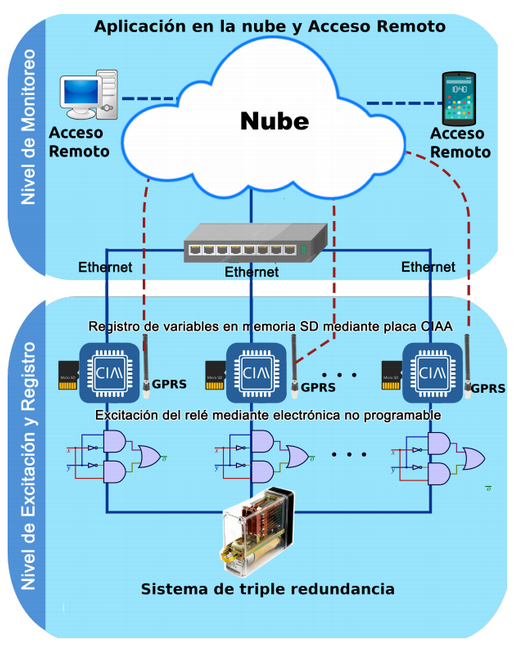
\includegraphics[width=.6\textwidth]{./Figuras/bloques.png}
\caption{Diagrama en bloques del sistema}
\label{fig:diagBloques2}
\end{figure}

\vspace{25px}

El firmware correrá sobre 3 placas CIAA-NXP en simultáneo para asegurar los niveles de disponibilidad deseados. Sobre cada una de las CIAA-NXP se monta una placa de lógica no programable. Este subsistema cuenta entre otras con las siguientes funciones:

\begin{itemize}
\item Generar la señal de activación del relé (incluyendo los transistores de potencia y circuitos de activación correspondientes).
\item Realizar la sincronización automática de las señales de activación del relé generadas por tres placas independientes entre sí.
\item Detectar cuando una de las tres placas falla y en ese caso desconectarla del relé en forma automática.
\item Realizar la medición de múltiples valores de voltaje y corriente asociados al funcionamiento del relé. Estos valores son el voltaje aplicado al bobinado del relé y la corriente que circula, junto con los valores de voltaje aplicado y la corriente que circula por cada contacto. Se ensayarán relés que usualmente cuentan con hasta seis contactos normal cerrado y seis contactos normal abierto.
\item Mostrar indicaciones luminosas relativas al estado del sistema mediante diodos LED.
\item Establecer una comunicación MQTT sobre TCP/IP con el broker para recibir los comandos del usuario y enviar, en tiempo real, los datos recabados.
\end{itemize}

Para cumplir con los requerimientos de la norma, el sistema debe ser capaz de realizar los siguientes ensayos:

\begin{itemize}
\item \textbf{Sistema magnético, corriente de excitación y corriente de caída:} la corriente de excitación se define como la corriente mínima a través de la bobina que, partiendo de un valor nulo, alcanza para mover la armadura de la posición de reposo a la posición de trabajo y para aplicar la fuerza de contacto especificada por el fabricante, cerrando todos los contactos de trabajo. La corriente de caída es la corriente máxima a través de la bobina que, partiendo del valor de la corriente nominal, produce la apertura de todos los contactos de trabajo. Este ensayo permite medir el factor K. Para esto se debe generar una función de rampa que, luego de ser amplificada, se aplica al bobinado del relé.
\item \textbf{Ensayo de vida útil mecánica:} este ensayo es en vacío. El usuario puede ingresar la cantidad de ciclos a ensayar siendo el valor máximo de $10 \cdot 10^6$ movimientos porque la norma se cumple cuando se llega esta cantidad de ciclos. Este ensayo registra la corriente y el voltaje del bobinado y el estado de los contactos.
\item \textbf{Ensayo con carga:} este ensayo se realiza aplicando el voltaje nominal los contactos abiertos y la corriente nominal a los contactos cerrados. A la bobina del relé también se le aplica el voltaje nominal. La norma dice que en estas condiciones se debe asegurar una cantidad mínima de $2 \cdot 10^6$ movimientos durante la vida útil del relé. En este ensayo se registran los voltajes y las corrientes de la bobina y los voltajes y las corrientes de los contactos.
\end{itemize}

\section{Identificación y análisis de los interesados}
\label{sec:interesados}

\begin{table}[H]
%\caption{Identificación de los interesados}
%\label{tab:interesados}
\begin{tabularx}{\linewidth}{@{}|l|X|X|l|@{}}
\hline
\rowcolor[HTML]{C0C0C0} 
Rol           & Nombre y Apellido & Organización 	  & Puesto 	\\ \hline
Cliente       & \clientename      &\empclientename	  & \shortstack {Coordinador General\\de Desarrollo,\\de la Subgerencia\\de Desarrollo y\\Normas Técnicas}\\ \hline
Responsable   & \authorname       & CESE 12Co2020 	  & Alumno 	\\ \hline
Orientador    & \supname	       & \pertesupname 	  & Director	Trabajo final \\ \hline
\multirow{2}{*}{Colaboradores} & Ing. Nicolás Locatelli & CONICET-GICSAFe & \shortstack[l]{Integrante} \\ \cline{2-4}
& Ing. Gustavo Ramoscelli & CONICET-GICSAFe & \shortstack[l]{Investigador} \\ \hline
\end{tabularx}
\textbf{CONICET-GICSAFe:} Grupo de Investigación en Calidad y Seguridad de las Aplicaciones Ferroviarias
\end{table}

\section{1. Propósito del proyecto}
\label{sec:proposito}

El propósito de este proyecto es desarrollar el firmware para un probador de relés de seguridad ferroviarios. El mismo deberá comunicarse con un servidor remoto, desde el cuál se configurarán e iniciarán las pruebas. Además, deberá reportar en tiempo real el estado de las pruebas, junto con las mediciones que la conforman.

\section{2. Alcance del proyecto}
\label{sec:alcance}

Se diseñará e implementará el firmware capaz de realizar, junto con el hardware, las tres pruebas mencionadas anteriormente en la descripción técnica del proyecto. 
En la entrega final no se incluirá el desarrollo de hardware del probador ni el software del servidor remoto.

\section{3. Supuestos del proyecto}
\label{sec:supuestos}

\begin{itemize}
\item Se contará con el hardware terminado al arrancar con el desarrollo de firmware.
\item Se dispondrá, en una etapa avanzada del desarrollo, de un servidor de pruebas con las funcionalidades mínimas requeridas por el probador.
\end{itemize}

\section{4. Requerimientos}
\label{sec:requerimientos}

\begin{enumerate}
\item Interfaces Externas
	\begin{enumerate}
	\item El firmware deberá ser capaz de leer el estado de 5 señales digitales.
	\item El firmware deberá leer 15 señales analógicas a través de 2 integrados ADC externos.
	\item El firmware deberá leer 2 señales analógicas a través de 2 ADC internos.
	\item El firmware deberá leer el estado de un pin digital.
	\item El firmware deberá controlar el estado de 2 pines digitales.
	\item El firmware deberá comunicarse con la tarjeta MicroSD presente en el hardware.
	\item El firmware deberá hacer uso de un puerto Ethernet para conectarse a Internet.
	\item El firmware deberá ser capaz de generar una rampa de tensión configurable.
	\end{enumerate}
\item Funciones
	\begin{enumerate}
	\item El firmware debe ser capaz de enviar notificaciones de alerta al servidor remoto, generadas por el disparo de una señal de alerta del hardware.
	\item El firmware debe ser capaz de enviar notificaciones de alerta al servidor remoto, generadas por sobretensión en cualquiera de las entradas analógicas.
	\item El firmware debe ser capaz de interpretar los siguientes comandos enviados desde el servidor:
		\begin{enumerate}
		\item Aplicar configuración de sistema.
		\item Definir los parámetros asociados a cada tipo de ensayo.
		\item Disparar ensayos.
		\item Parar ensayos.
		\end{enumerate}
	\item El firmware deberá ser capaz de ejecutar los siguientes ensayos:
		\begin{enumerate}
		\item \textbf{Sistema magnético, corriente de excitación y corriente de caída:} Se genera una rampa de tensión de pendiente positiva y luego otra de pendiente negativa. El valor inicial, valor final, paso de tensión y duración del paso de las señales deben ser configurables en ambos casos, además de la máxima corriente de excitación admitida. Se debe notificar al servidor entre paso y paso, indicando la tensión instantánea de la rampa y el valor de las 17 señales analógicas. La prueba finaliza al completarse la cantidad de repeticiones especificadas al inicio de la prueba.
		\item \textbf{Ensayo de vida útil mecánica con y sin carga:} Se debe especificar el número de ciclos. Al detectarse la secuencia de inicio se comienzan a contabilizar los ciclos, representados por el periodo entre cada secuencia de inicio. Se debe notificar al servidor cada vez que ocurre un flanco positivo de las señales CLOCK\_1S o CLOCK\_3S, indicando el número de ciclo y el valor de las 17 señales analógicas. La prueba finaliza al completarse la cantidad de ciclos especificados al inicio de la prueba.
		\end{enumerate}
	\item Junto con cada paquete de datos generado a partir de una prueba, se debe anexar un ID que identifique el tipo de prueba.
	\item Junto con cada paquete de datos se debe anexar una marca temporal y un ID que identifique a la placa dentro de las tres placas que conforman el sistema.
	\item Cada paquete de datos debe ser almacenado en una tarjeta MicroSD a modo de copia de seguridad.
	\item El firmware debe permitir realizar distintos tipos de ensayos en forma intercalada.
	\item El firmware debe permitir configurar los siguientes parámetros:
		\begin{enumerate}
		\item Hora del sistema.
		\item URL y puerto del broker MQTT.
		\end{enumerate}
	\end{enumerate}
\item Requisitos de Rendimiento
	\begin{enumerate}
	\item Para el ensayo de rampa se deben permitir hasta 25 ciclos.
	\item Para el ensayo de vida útil mecánica \textbf{sin carga} se deben permitir hasta $10 \cdot 10^6$ ciclos.
	\item Para el ensayo de vida útil mecánica \textbf{con carga} se deben permitir hasta $2 \cdot 10^6$ ciclos.
	\item Para el ensayo de vida útil mecánica el periodo máximo entre ciclos es de 3 segundos.
	\end{enumerate}
\item Restricciones de Diseño
	\begin{enumerate}
	\item Se usará I$^2$C como protocolo de comunicación con los ADC.
	\item Se usará SPI como protocolo de comunicación con la SD.
	\item Se usará MQTT sobre TCP/IP como protocolo de comunicación con el servidor remoto.
	\item Se usará JSON como formato de texto para intercambio de datos con el servidor remoto.
	\item La rampa de tensión debe ser capaz de alcanzar un valor máximo de hasta 10V.
	\item Se usará la plataforma CIAA-NXP como placa de desarrollo.
	\item Se usará un RTC para mantener la hora de forma local.
	\item Se usará ``Unix time'' como formato de marca temporal. 
	\end{enumerate}
\item Atributos del Sistema
	\begin{enumerate}
	\item El firmware debe ser capaz de recuperarse ante una falla que provoque el reinicio del microcontrolador, en un tiempo menor a los 3 segundos y retomar los ensayos en curso.
	\item El firmware debe hacer uso de cifrado TLS para la capa de transporte.
	\item El firmware debe hacer uso de Usuario/Contraseña para autenticarse con el broker MQTT.
	\item El desarrollo de software debe seguir una metodología acorde a la norma UNE-EN 50128.
	\end{enumerate}
\item Otros Requisitos
	\begin{enumerate}
	\item El desarrollo debe ser documentado utilizando la herramienta Doxygen.
	\end{enumerate}
\end{enumerate}

%\subsubsection*{4.1 Especificación de formato de archivos JSON}
%\label{sec:espec_json}
%
%A continuación se detallan los pares nombre/valor para los distintos archivos JSON que se intercambiarán entre firmware y servidor. Algunos son comunes a todos los mensajes mientras que otros dependen del comando en cuestión.
%
%\textbf{Pares nombre/valor comunes a todos los JSON:}
%
%\textbf{``board\_id''}\textit{(integer)}: Número de placa.\\
%\textbf{``cmd''}\textit{(string)}: Cadena que identifica al comando. Los posibles comandos son: \\
%	\forceindent test\_config = Configuración del ensayo.\\
%	\forceindent test\_start = Disparo del ensayo.\\
%	\forceindent test\_stop = Parada del ensayo.\\
%\textbf{``params''}\textit{(object)}: Dentro de este objeto se anidan los parámetros asociados al comando. \\
%
%\textbf{Parámetros específicos:}
%
%\underline{\Large test\_config:}\\
%\textbf{``type''}\textit{(integer)}: Tipo de ensayo.\\
%	\forceindent 1 = Sistema magnético, corriente de excitación y corriente de caída.\\
%	\forceindent 2 = Ensayo de vida útil mecánica sin carga.\\
%	\forceindent 3 = Ensayo de vida útil mecánica con carga.\\
%\textbf{``cycles''}\textit{(integer)}: Número de ciclos a repetir.\\
%{\large - Parámetros específicos del ensayo tipo 1:}\\
%\textbf{``vem''}\textit{(integer)}: Tensión máxima de la rampa [V].\\
%\textbf{``inom''}\textit{(integer)}: Corriente nominal [mA].\\
%\textbf{``step''}\textit{(integer)}: Salto de voltaje [mV].\\
%\textbf{``dt''}\textit{(integer)}: Duración del paso [ms].\\
%\textbf{``ip\_max''}\textit{(integer)}: Máxima corriente de excitación admitida [mA].\\
%
%\underline{\Large test\_start:}\\
%\textbf{``type''}\textit{(integer)}: Tipo de ensayo.\\


\section{5. Entregables principales del proyecto}
\label{sec:entregables}

\begin{itemize}
\item Código fuente del firmware
\item Informe de avance
\item Memoria del trabajo
\item Informes de ensayos
\end{itemize}

\section{6. Desglose del trabajo en tareas}
\label{sec:wbs}

\begin{enumerate}
\item Planificación \hfill (55 hs)
	\begin{enumerate}
	\item Estudio del funcionamiento básico de un probador. \hfill (25 hs)
	\item Elaboración del documento de Planificación del proyecto. \hfill (30 hs)
	\end{enumerate}
\item Pruebas preliminares \hfill (80 hs)
	\begin{enumerate}
	\item Desarrollo del prototipo de firmware. \hfill (25 hs)
	\item Pruebas de interacción con el hardware. \hfill (35 hs)
	\item Pruebas de comunicación con el servidor. \hfill (20 hs)
	\end{enumerate}
\item Diseño de firmware \hfill (100 hs)
	\begin{enumerate}
	\item Diseño de la arquitectura general y el flujo de datos. \hfill (35 hs)
	\item Diseño de las tareas del RTOS y los mecanismos \newline de comunicación entre ellas.  \hfill (35 hs)
	\item Configuración del entorno de desarrollo. \hfill (15 hs)
	\item Estudio de las herramientas de software disponibles para la plataforma \newline de desarrollo elegida. \hfill (15 hs)
	\end{enumerate}
\item Implementación de firmware \hfill (229 hs)
	\begin{enumerate}
	\item Desarrollo del driver para los ADC. \hfill (25 hs)
	\item Desarrollo del módulo de adquisición. \hfill (32 hs)
	\item Desarrollo del driver ethernet. \hfill (40 hs)
	\item Desarrollo del módulo de comunicación. \hfill (40 hs)
	\item Desarrollo del módulo de almacenamiento SD.  \hfill (32 hs)
	\item Desarrollo del módulo de detección de estados. \hfill (20 hs)
	\item Desarrollo del módulo de control principal. \hfill (40 hs)
	\end{enumerate}
\item Verificación y Validación \hfill (163 hs)
	\begin{enumerate}
	\item Pruebas individuales de los módulos de firmware.  \hfill (30 hs)
	\item Ensayos de integración del firmware.  \hfill (20 hs)
	\item Pruebas de integración con el hardware. \hfill (20 hs)
	\item Ensayos funcionales. \hfill (40 hs)
	\item Análisis de los efectos de los errores de software. \hfill (20 hs)
	\item Demostración formal. \hfill (8 hs)
	\item Elaboración del informe de validación. \hfill (25 hs)
	\end{enumerate}
\item Documentación \hfill (60 hs)
	\begin{enumerate}
	\item Elaboración de la Memoria del trabajo. \hfill (40 hs)
	\item Producción de la presentación final. \hfill (20 hs)
	\end{enumerate}
\end{enumerate}

Cantidad total de horas: (687 hs)

\section{7. Diagrama de Activity On Node}
\label{sec:AoN}

\begin{figure}[H]
\centering 
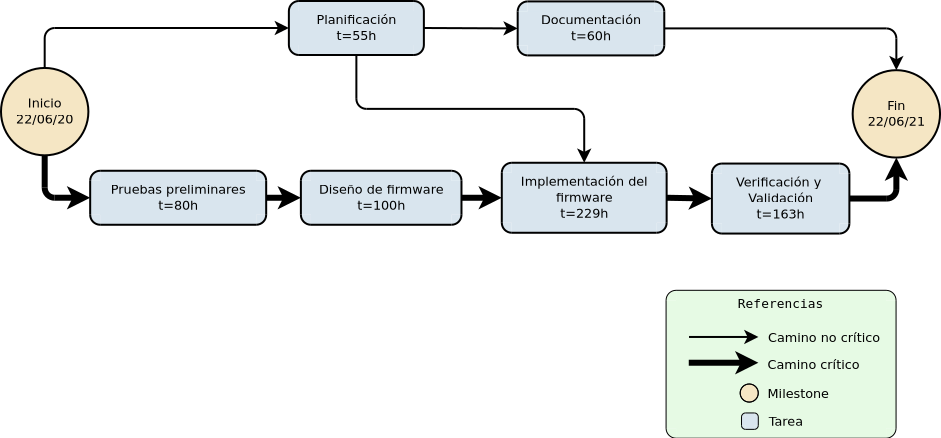
\includegraphics[width=.8\textwidth]{./Figuras/AoN2.png}
\caption{Diagrama en \textit{Activity on Node}}
\label{fig:AoN}
\end{figure}

\section{8. Diagrama de Gantt}
\label{sec:gantt}

\begin{center}
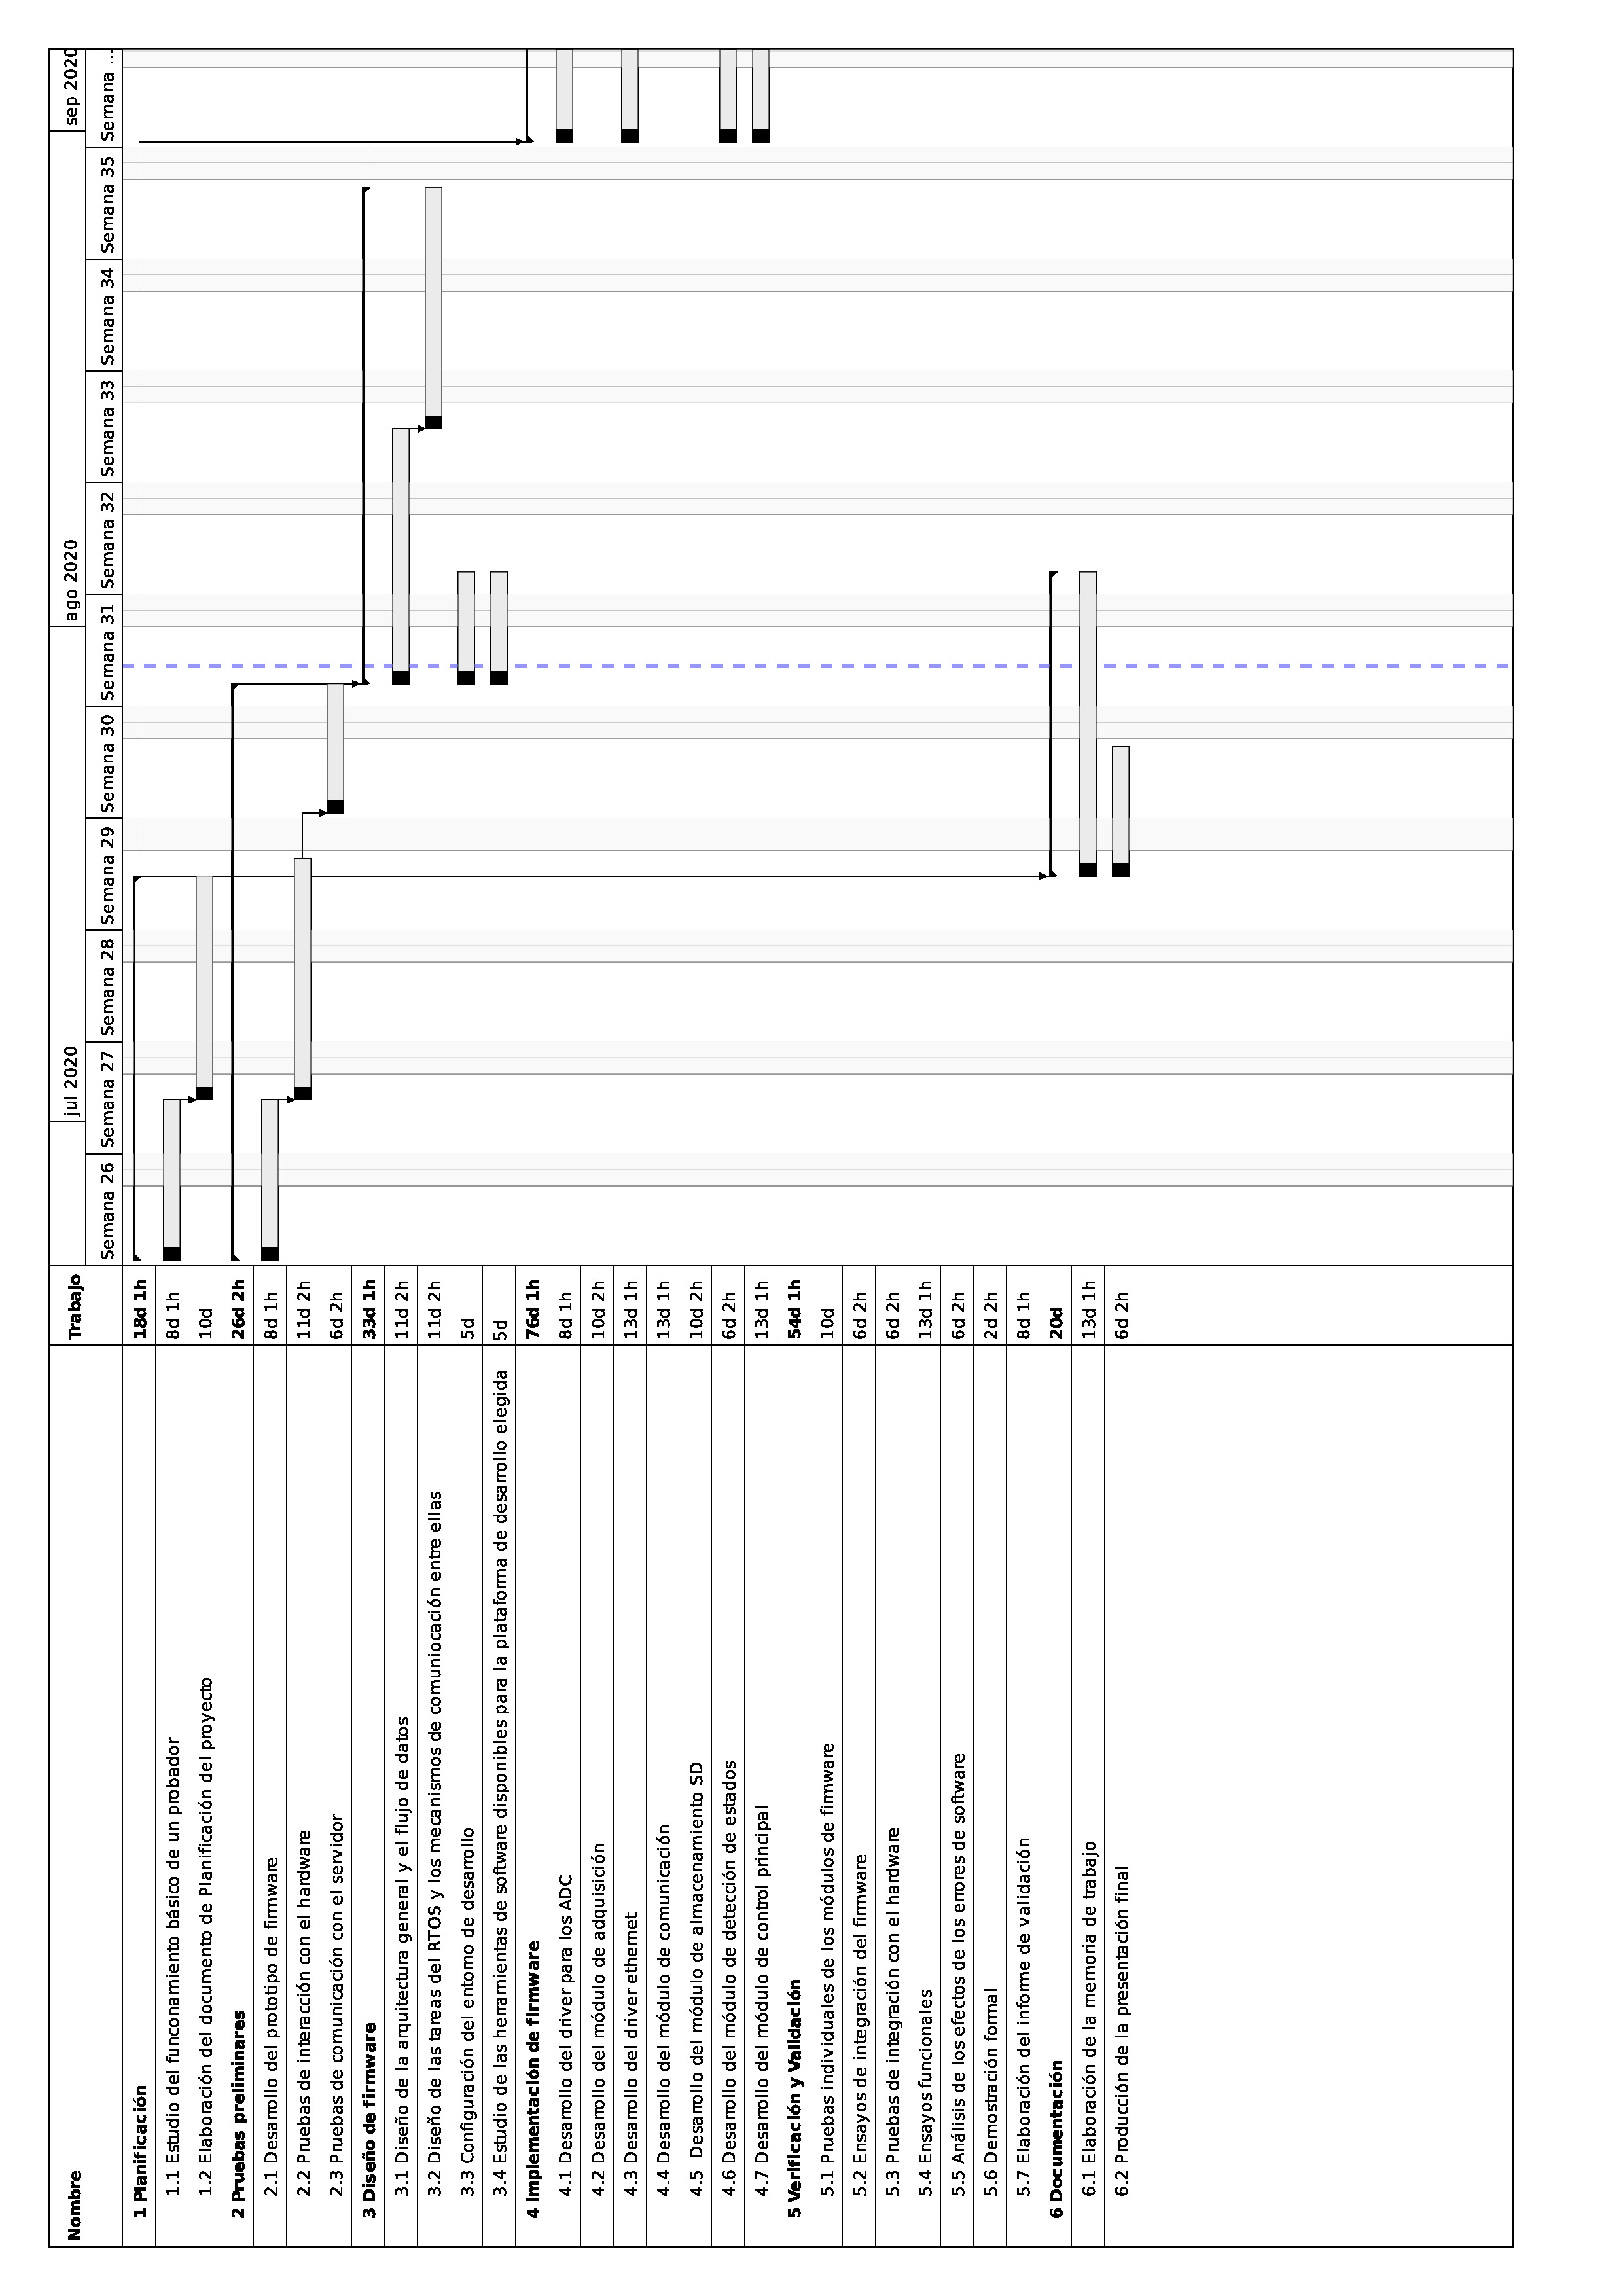
\includegraphics[width=0.95\textwidth, angle=180]{./Figuras/gantt-0.jpg}
\captionof{figure}{Diagrama de gantt}
\label{fig:gantt}
\end{center}

\begin{center}
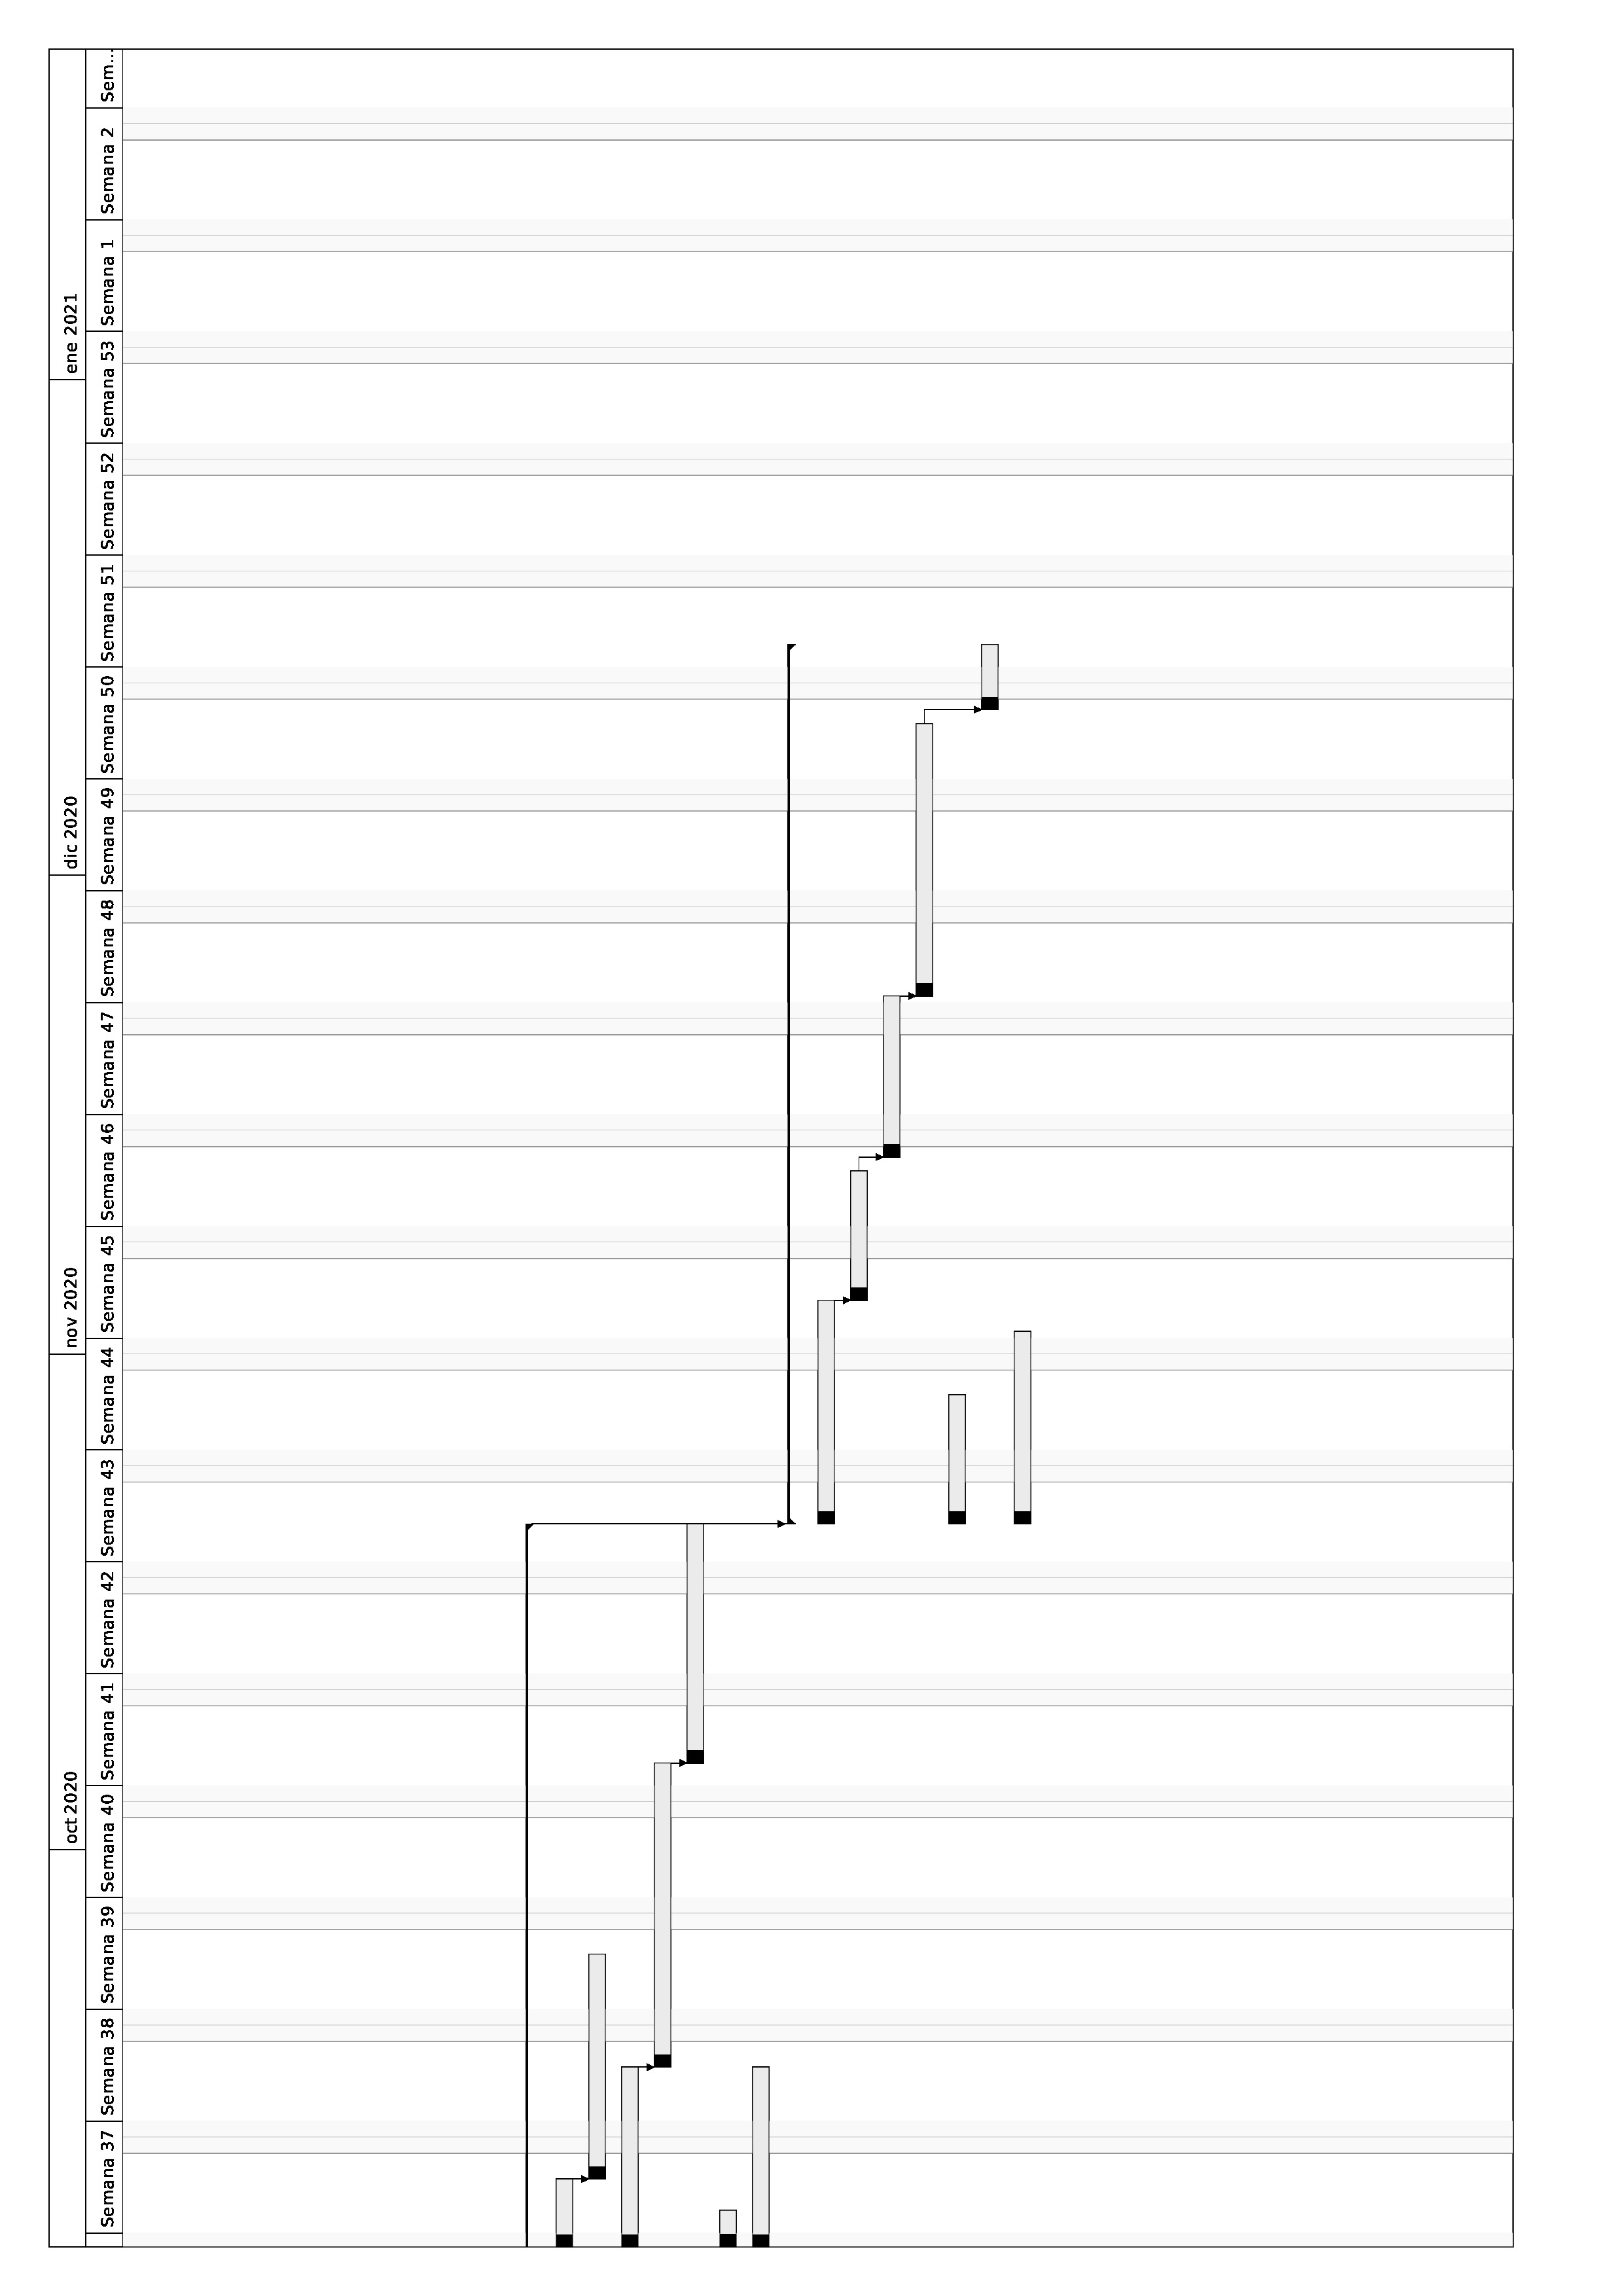
\includegraphics[width=0.95\textwidth, angle=180]{./Figuras/gantt-1.jpg}
\captionof{figure}{Diagrama de gantt (continuación)}
\label{fig:gantt}
\end{center}

\section{9. Matriz de uso de recursos de materiales}
\label{sec:recursos}

\begin{table}[H]
\label{tab:recursos}
\centering
\begin{tabularx}{\linewidth}{@{}|c|X|c|c|@{}}
\hline
\cellcolor[HTML]{C0C0C0} & \cellcolor[HTML]{C0C0C0} & \multicolumn{2}{c|}{\cellcolor[HTML]{C0C0C0}Recursos requeridos (horas)} \\ \cline{3-4} 
\multirow{-2}{*}{\cellcolor[HTML]{C0C0C0}WBS} & \multirow{-2}{*}{\cellcolor[HTML]{C0C0C0}\begin{tabular}[c]{@{}c@{}}Nombre de la tarea\end{tabular}} & PC & Probador+CIAA \\ \hline
 1.1 & Estudio del funcionamiento básico de un probador & 25 & 10 \\ \hline
 1.2 & Elaboración del documento de planificación del proyecto & 30 & \\ \hline
 2.1 & Desarrollo del prototipo de firmware & 25 & 10 \\ \hline
 2.2 & Pruebas de interacción con el hardware & 35 & 10\\ \hline
 2.3 & Pruebas de comunicación con el servidor & 20 & \\ \hline
 3.1 & Diseño de la arquitectura general y el flujo de datos & 35 & \\ \hline
 3.2 & Diseño de las tareas del RTOS y los mecanismos de comunicación entre ellas & 35 & \\ \hline
 3.3 & Configuración del entorno de desarrollo & 15 & \\ \hline
 3.4 & Estudio de las herrameintas de software disponible para la plataforma de desarrollo elegida & 15 & \\ \hline
 4.1 & Desarrollo del driver para los ADC & 25 & 15 \\ \hline
 4.2 & Desarrollo del módulo de adquisición & 32 & 5 \\ \hline
 4.3 & Desarrollo del driver ethernet & 40 & 5 \\ \hline
 4.4 & Desarrollo del módulo de comunicación & 40 & \\ \hline
 4.5 & Desarrollo del módulo de almacenamiento SD & 32 & 5 \\ \hline
 4.6 & Desarrollo del módulo de detección de estados & 20 & 5 \\ \hline
 4.7 & Desarrollo del módulo de control principal & 40 & \\ \hline
 5.1 & Pruebas individuales de los módulos de firmware & 30 & 10 \\ \hline
 5.2 & Ensayos de integración del firmware & 20 & 20 \\ \hline
 5.3 & Pruebas de integración con el hardware & 20 & 20 \\ \hline
 5.4 & Ensayos funcionales & 40 & 40 \\ \hline
 5.5 & Análisis de los efectos de los errores de software 20 & 15 & \\ \hline
 5.6 & Demostración formal & 8 & 8 \\ \hline
 5.7 & Elaboración del informe de validación & 25 & \\ \hline 
 6.1 & Elaboración de la memoria de trabajo & 40 & \\ \hline 
 6.2 & Producción de la presentación final & 20 & \\ \hline 
\end{tabularx}%
\end{table}


\section{10. Presupuesto detallado del proyecto}
\label{sec:presupuesto}

\begin{table}[H]
\centering
\begin{tabularx}{\linewidth}{@{}|X|c|r|r|@{}}
\hline
\rowcolor[HTML]{C0C0C0} 
\multicolumn{4}{|c|}{\cellcolor[HTML]{C0C0C0}COSTOS DIRECTOS} \\ \hline
\rowcolor[HTML]{C0C0C0} 
Descripción &
  \multicolumn{1}{c|}{\cellcolor[HTML]{C0C0C0}Cantidad} &
  \multicolumn{1}{c|}{\cellcolor[HTML]{C0C0C0}Valor unitario} &
  \multicolumn{1}{c|}{\cellcolor[HTML]{C0C0C0}Valor total} \\ \hline
CIAA-NXP                    & 1        & \$ 25.600  & \$ 25.600  \\  \hline
Poncho Probador de relés    & 1        & \$ 12.693  & \$ 12.693  \\ \hline
Transformador 220VAC/12VAC  & 1        & \$ 918     & \$ 918     \\ \hline
Mano de obra                & 687 hs   & \$ 850     & \$ 583.950 \\ \hline
\multicolumn{3}{|c|}{SUBTOTAL} &
  \multicolumn{1}{c|}{\$ 622.243} \\ \hline
\rowcolor[HTML]{C0C0C0} 
\multicolumn{4}{|c|}{\cellcolor[HTML]{C0C0C0}COSTOS INDIRECTOS} \\ \hline
\rowcolor[HTML]{C0C0C0}
Descripción &
  \multicolumn{1}{c|}{\cellcolor[HTML]{C0C0C0}Cantidad} &
  \multicolumn{1}{c|}{\cellcolor[HTML]{C0C0C0}Valor unitario} &
  \multicolumn{1}{c|}{\cellcolor[HTML]{C0C0C0}Valor total} \\ \hline
30\% de los costos directos & N/A & N/A & \$ 186.673  \\  \hline
\multicolumn{3}{|c|}{SUBTOTAL} &
  \multicolumn{1}{c|}{} \\ \hline
\rowcolor[HTML]{C0C0C0}
\multicolumn{3}{|c|}{TOTAL} &
   \\ \hline
\end{tabularx}%
\end{table}


\section{11. Matriz de asignación de responsabilidades}
\label{sec:responsabilidades}

\begin{table}[htpb]
\centering
\resizebox{\textwidth}{!}{%
\begin{tabular}{|c|m{6cm}|c|c|c|c|c|}
\hline
\rowcolor[HTML]{C0C0C0} 
\cellcolor[HTML]{C0C0C0} &
  \cellcolor[HTML]{C0C0C0} &
  \multicolumn{5}{c|}{\cellcolor[HTML]{C0C0C0}Nombres y roles del proyecto} \\ \cline{3-6} 
\rowcolor[HTML]{C0C0C0} 
\cellcolor[HTML]{C0C0C0} &
  \cellcolor[HTML]{C0C0C0} &
  Responsable &
  Orientador &
  Colaborador &
  Colaborador &
  Cliente \\ \cline{3-6} 
\rowcolor[HTML]{C0C0C0} 
\multirow{-3}{*}{\cellcolor[HTML]{C0C0C0}\begin{tabular}[c]{@{}c@{}}Código\\ WBS\end{tabular}} &
  \multirow{-3}{*}{\cellcolor[HTML]{C0C0C0}Nombre de la tarea} &
  \authorname &
  \supname &
  Ing. Nicolás Locatelli &
  Ing. Gustavo Ramoscelli &
  \clientename \\ \hline
 1.1 & Estudio del funcionamiento básico de un probador & P & C & & & \\ \hline
 1.2 & Elaboración del documento de planificación del proyecto & P & A & & & I \\ \hline
 2.1 & Desarrollo del prototipo de firmware & P & C & & & \\ \hline
 2.2 & Pruebas de interacción con el hardware & P & C & & & \\ \hline
 2.3 & Pruebas de comunicación con el servidor & P & & C & C & \\ \hline
 3.1 & Diseño de la arquitectura general y el flujo de datos & P & & & & \\ \hline
 3.2 & Diseño de las tareas del RTOS y los mecanismos de comunicación entre ellas & P & & & & \\ \hline
 3.3 & Configuración del entorno de desarrollo & P & & & & \\ \hline
 3.4 & Estudio de las herrameintas de software disponible para la plataforma de desarrollo elegida & P & & & & \\ \hline
 4.1 & Desarrollo del driver para los ADC & P & C & & & \\ \hline
 4.2 & Desarrollo del módulo de adquisición & P & I & & & \\ \hline
 4.3 & Desarrollo del driver ethernet & P & & & & \\ \hline
 4.4 & Desarrollo del módulo de comunicación & P & & I & I & \\ \hline
 4.5 & Desarrollo del módulo de almacenamiento SD & P & I & & & \\ \hline
 4.6 & Desarrollo del módulo de detección de estados & P & C & & & \\ \hline
 4.7 & Desarrollo del módulo de control principal & P & I & & & \\ \hline
 5.1 & Pruebas individuales de los módulos de firmware & P & & & & \\ \hline
 5.2 & Ensayos de integración del firmware & P & I & & & \\ \hline
 5.3 & Pruebas de integración con el hardware & P & A & & & \\ \hline
 5.4 & Ensayos funcionales & P & A & A & A & A \\ \hline
 5.5 & Análisis de los efectos de los errores de software & P & C & & & \\ \hline
 5.6 & Demostración formal & P & A & I & I & A \\ \hline
 5.7 & Elaboración del informe de validación & P & A & & & \\ \hline 
 6.1 & Elaboración de la memoria de trabajo & P & A & & & \\ \hline 
 6.2 & Producción de la presentación final & P & A & & & \\ \hline 
\end{tabular}%
}
\end{table}

{\footnotesize
Referencias:
\begin{itemize}
	\item P = Responsabilidad Primaria
	\item S = Responsabilidad Secundaria
	\item A = Aprobación
	\item I = Informado
	\item C = Consultado
\end{itemize}
} %footnotesize

\section{12. Gestión de riesgos}
\label{sec:riesgos}

\subsection*{12.1. Identificación de riesgos y estimación de sus consecuencias}

\begin{tcolorbox}
\textbf{Riesgo 1: avería de la CIAA o del poncho}
\begin{itemize}
	\item \textit{Severidad: 8} - Dificultaría la implementación del firmware y sería necesario reponer el hardware para continuar con el desarrollo.
	\item \textit{Ocurrencia: 2} - Solo se interactuará con el hardware a través del firmware. Es poco probable que se dañe el equipamiento.
\end{itemize}
\end{tcolorbox}

\begin{tcolorbox}
\textbf{Riesgo 2: Errores en el diseño de hardware del probador}
\begin{itemize}
	\item \textit{Severidad: 6} - Dificultaría las pruebas para validar el correcto funcionamiento del firmware. 
	\item \textit{Ocurrencia: 2} - El hardware fue probado exhaustivamente, por lo que es poco probable que surjan nuevos errores de diseño.
\end{itemize}
\end{tcolorbox}

\begin{tcolorbox}
\textbf{Riesgo 3: Demoras en los tiempos estipulados para cada tarea}
\begin{itemize}
	\item \textit{Severidad: 6} - Retrasaría el desarrollo del proyecto. Sin embargo se cuenta con márgenes de tiempo, por lo que no sería un problema, siempre y cuando las demoras no sean excesivas.
	\item \textit{Ocurrencia: 8} - Dada la poca experiencia en planificación de proyectos, existe una alta probabilidad de que los tiempos no hayan sido correctamente estimados.
\end{itemize}
\end{tcolorbox}

\begin{tcolorbox}
\textbf{Riesgo 4: Dificultades en el desarrollo del driver de red}
\begin{itemize}
	\item \textit{Severidad: 10} - Se estima que el driver de red junto con el stack TCP/IP es el módulo mas complejo en todo el diseño. No lograr implementar dicho módulo haría imposible conseguir los objetivos planteados.
	\item \textit{Ocurrencia: 2} - Si bien el manejo del hardware de red se presenta como una tarea compleja, se cuenta con el soporte de la comunidad de desarrolladores en torno a la CIAA.
\end{itemize}
\end{tcolorbox}

\begin{tcolorbox}
\textbf{Riesgo 5: No lograr que el firmware cumpla con los requisitos de rendimiento}
\begin{itemize}
	\item \textit{Severidad: 8} - En caso de que no se logre realizar la lectura de todas las señales analógicas y el envío del paquete al servidor entre ciclo y ciclo, será necesario recurrir a un microprocesador de mayores prestaciones.
	\item \textit{Ocurrencia: 2} - Se estima que el microprocesador de la CIAA-NXP cuenta con capacidad de sobra para realizar las tareas mencionadas con la frecuencia requerida.
\end{itemize}
\end{tcolorbox}

\subsection*{12.2. Tabla de gestión de riesgos}

\begin{table}[htpb]
\centering
\begin{tabularx}{\linewidth}{@{}|c|X|c|c|c|c|c|c|@{}}
\hline
\rowcolor[HTML]{C0C0C0} 
Riegos & Detalle                                                            & S  & O & RPN & S* & O* & RPN* \\ \hline
1      & Avería de la CIAA o el poncho                                      & 8  & 2 & 16  &    &    &      \\ \hline
2      & Errores en el diseño de hardware del probador                      & 6  & 2 & 12  &    &    &      \\ \hline
3      & Demoras en los tiempos estipulados para cada tarea                 & 6  & 8 & 48  & 6  & 4  & 24   \\ \hline
4      & Dificultades en el desarrollo del driver de red                    & 10 & 2 & 20  &    &    &      \\ \hline
5      & No lograr que el firmware cumpla con los requisitos de rendimiento & 8  & 2 & 16  &    &    &      \\ \hline
\end{tabularx}%
\end{table}

Criterio adoptado: 
Se tomarán medidas de mitigación en los riesgos cuyos números de RPN sean mayores a \textbf{40}.

Nota: los valores marcados con (*) en la tabla corresponden luego de haber aplicado la mitigación.

\subsection*{12.3. Plan de mitigación de riesgos}

\begin{tcolorbox}
\textbf{Riesgo 3: Demoras en los tiempos estipulados para cada tarea}
\begin{itemize}
	\item \textit{Plan de mitigación: } Reveer el plan de trabajo y aumentar las horas dedicadas al proyecto.
	\item \textit{Severidad: 6} - Retrasaría el desarrollo del proyecto. Sin embargo se cuenta con márgenes de tiempo, por lo que no sería un problema, siempre y cuando las demoras no sean excesivas. Se mantiene la severidad.
	\item \textit{Ocurrencia: 4} - Si se aumentan las horas de trabajo disminuye la probabilidad de tener demoras.
\end{itemize}
\end{tcolorbox}

\section{13. Gestión de la calidad}
\label{sec:calidad}

\begin{tcolorbox}
\textit{1. Interfaces Externas} \\ \\
	\textbf{Verificación:} Durante la fase de Pruebas preliminares, se desarrollará un prototipo de firmware que haga uso de todos los periféricos mencionados. De esta forma se verificará el correcto funcionamiento de los mismos. \\
	\textbf{Validación:} Se mostrará este firmware funcionando al \supname , quién validará o no el funcionamiento de los periféricos. \\
\end{tcolorbox}

\begin{tcolorbox}	
\textit{2.1 El firmware debe ser capaz de enviar notificaciones de alerta al servidor remoto, generadas por el disparo de una señal de alerta del hardware.} \\ \\
\textit{2.2 El firmware debe ser capaz de enviar notificaciones de alerta al servidor remoto, generadas por sobretensión en cualquiera de las entradas analógicas.} \\ 	\\
\textit{2.3 El firmware debe ser capaz de interpretar los siguientes comandos enviados desde el servidor:
		\begin{itemize}
		\item Aplicar configuración de sistema.
		\item Definir los parámetros asociados a cada tipo de ensayo.
		\item Disparar ensayos.
		\item Parar ensayos. \\
		\end{itemize}}
	\textit{2.5 Junto con cada paquete de datos generado a partir de una prueba, se debe anexar un ID que identifique el tipo de prueba.} \\ \\
	\textit{2.6 Junto con cada paquete de datos se debe anexar una marca temporal y un ID que identifique a la placa dentro de las tres placas que conforman el sistema.} \\ \\
	\textit{2.9 El firmware debe permitir configurar los siguientes parámetros:
		\begin{itemize}
		\item Hora del sistema.
		\item URL y puerto del broker MQTT. \\
		\end{itemize}}
	\textbf{Verificación:} Se acordará con los Ingenieros Gustavo Ramoscelli y Nicolás Locatelli, encargados del desarrollo de la aplicación servidor, las pruebas a realizar para el envío de mensajes de alerta, así como la recepción por parte del firmware de los comandos mencionados. \\
	\textbf{Validación:} Una vez realizada la verificación y con el firmware completamente implementado, en el marco de los Ensayos funcionales, se validará la comunicación con el servidor. \\
\end{tcolorbox}

\begin{tcolorbox}
	\textit{2.4 El firmware deberá ser capaz de ejecutar los siguientes ensayos: (ver requerimientos)} \\ \\
	\textit{2.8 El firmware debe permitir realizar distintos tipos de ensayos en forma intercalada.} \\ \\
	\textbf{Verificación:} Se conectará un relé de baja intensidad en los terminales de prueba y se corroborará que las secuencias de ensayo se desarrollen correctamente. \\
	\textbf{Validación:} Se conectará el hardware en su totalidad y se lo hará funcionar durante un tiempo prolongada, verificando en todo momento el correcto funcionamiento del mismo. \\
\end{tcolorbox}

\begin{tcolorbox}
	\textit{2.7 Cada paquete de datos debe ser almacenado en una tarjeta MicroSD a modo de copia de seguridad.} \\ \\
	\textbf{Verificación:} Al finalizar las pruebas de verificación del requerimiento 2.4, se corroborará que los archivos almacenados en la SD y los datos almacenados en el servidor coincidan. \\
	\textbf{Validación:} Se llevará a cabo el mismo procedimiento que para la verificación pero con la totalidad del hardware funcionando. \\
\end{tcolorbox}

\begin{tcolorbox}
	\textit{3.1 Para el ensayo de rampa se deben permitir hasta 25 ciclos.} \\ \\	
	\textit{3.2 Para el ensayo de vida útil mecánica \textbf{sin carga} se deben permitir hasta $10 \cdot 10^6$ ciclos.} \\ \\
	\textit{3.3 Para el ensayo de vida útil mecánica \textbf{con carga} se deben permitir hasta $2 \cdot 10^6$ ciclos.} \\ \\
	\textit{3.4 Para el ensayo de vida útil mecánica el periodo máximo entre ciclos es de 3 segundos.} \\ \\
	\textbf{Verificación:} Se verificará por revisión de diseño que el firmware sea capaz de manejar la cantidad máxima estipulada de ciclos. Para ello se tendrá en cuenta el tamaño de las variables utilizadas, además del diseño de los algoritmos encargados del control de los ensayos. \\
	\textbf{Validación:} - \\
\end{tcolorbox}

\begin{tcolorbox}	
	\textit{5.1 El firmware debe ser capaz de recuperarse ante una falla que provoque el reinicio del microcontrolador, en un tiempo menor a los 3 segundos y retomar los ensayos en curso.} \\ \\
	\textbf{Verificación:} Se corroborará que el tiempo de inicialización del firmware sea menor al estipulado. \\
	\textbf{Validación:} Se producirán fallas intencionales que provoquen el reinicio del microcontrolador y se medirá el tiempo necesario para dicho reinicio.\\
\end{tcolorbox}	

\begin{tcolorbox}	
	\textit{5.2 El firmware debe hacer uso de cifrado TLS para la capa de transporte.} \\ \\
	\textit{5.3 El firmware debe hacer uso de Usuario/Contraseña para autenticarse con el broker MQTT.} \\ \\
	\textbf{Verificación:} Una vez configurado el servidor para que solo acepte conexiones que utilicen cifrado TLS y el broker para que utilice autenticación por Usuario/Contraseña, se intentará establecer comunicación con el mismo. \\
	\textbf{Validación:} Se utilizará la herramienta de software Wireshark para corroborar que los paquetes enviados desde el firmware estén cifrados. \\
\end{tcolorbox}
	
\begin{tcolorbox}
	\textit{6.1 El desarrollo debe ser documentado utilizando la herramienta Doxygen.} \\ \\
	\textbf{Verificación:} Se irán generando documentaciones intermedias a lo largo del desarrollo. \\
	\textbf{Validación:} Al finalizar el desarrollo se generará la documentación en alguno de los formatos soportados por la herramienta. \\
\end{tcolorbox}


\section{14. Comunicación del proyecto}
\label{sec:comunicaciones}

A continuación se detalla el plan de comunicación del proyecto:

% Please add the following required packages to your document preamble:
% \usepackage{graphicx}
% \usepackage[table,xcdraw]{xcolor}
% If you use beamer only pass "xcolor=table" option, i.e. \documentclass[xcolor=table]{beamer}
\begin{table}[H]
\centering
\resizebox{\textwidth}{!}{%
\begin{tabular}{|m{3cm}|m{3cm}|m{3cm}|c|c|c|}
\hline
\rowcolor[HTML]{C0C0C0} 
\multicolumn{6}{|c|}{\cellcolor[HTML]{C0C0C0}PLAN DE COMUNICACIÓN DEL PROYECTO}           \\ \hline
\rowcolor[HTML]{C0C0C0} 
¿Qué comunicar? & Audiencia & Propósito & Frecuencia & Método de comunicac. & Responsable \\ \hline
Plan de Proyecto & Profesores de GdP, Director y Codirector del proyecto & Informar sobre el plan y la metodología de trabajo & Una única vez & Correo electrónico & \authorname \\ \hline
Desarrollo del módulo de red & Encargados del desarrollo web & Informar a los interesados sobre la disponibilidad del módulo de red para realizar pruebas & Una única vez & Correo electrónico & \authorname \\ \hline
Avances en las interfaces con el hardware & \supname & Verificar el correcto funcionamiento del hardware & Semanal & Correo electrónico & \authorname \\ \hline
Presentación final & Director y codirector del proyecto y director de la Especialización & Informar sobre la finalización del proyecto & Una única vez & Correo electrónico & \authorname \\ \hline
\end{tabular}%
}
\end{table}

\section{15. Gestión de Compras}
\label{sec:compras}

\textit{No se realizarán compras durante el desarrollo del proyecto.}

\section{16. Seguimiento y control}
\label{sec:seguimiento}

\begin{table}[H]
\centering
\begin{tabularx}{\linewidth}{@{}|c|m{5cm}|m{2cm}|X|X|@{}}
\hline
\rowcolor[HTML]{C0C0C0} 
\multicolumn{5}{|c|}{\cellcolor[HTML]{C0C0C0}SEGUIMIENTO DE AVANCE}                                                                       \\ \hline
\rowcolor[HTML]{C0C0C0} 
Tarea del WBS & Indicador de avance & Frecuencia de reporte & Persona a ser informada & Método de comunic. \\ \hline 
1.1 & Cantidad de documentos leídos & Semanal & \supname & Correo electrónico  \\ \hline
1.2 & Cantidad de secciones redactadas & Bimensual & \supname & Correo electrónico \\ \hline
2.1 & Cantidad de módulos implementados & Bimensual & \supname & Correo electrónico \\ \hline
2.2 & Interfaces de hardware testeadas & Semanal & \supname & Correo electrónico \\ \hline
2.3 & Cantidad archivos JSON implementados & Semanal & Ing. Gustavo Ramoscelli, Ing. Nicolás Locatelli & Grupo de chat \\ \hline
3.1 & Cantidad de módulos diseñados & Semanal & \cosupname & Correo electrónico \\ \hline
3.2 & Cantidad de tareas diseñadas & Semanal & \cosupname & Correo electrónico \\ \hline
3.3 & - & - & - & - \\ \hline
3.4 & - & - & - & - \\ \hline
4.1 & Cantidad de líneas de código escritas & Semanal & \cosupname , \supname & Correo electrónico \\ \hline
4.2 & Cantidad de líneas de código escritas & Semanal & \cosupname , \supname & Correo electrónico \\ \hline
4.3 & Cantidad de líneas de código escritas & Semanal & \cosupname & Correo electrónico \\ \hline
4.4 & Cantidad de líneas de código escritas & Semanal & \cosupname & Correo electrónico \\ \hline
\end{tabularx}%
%}
\end{table}

\begin{table}[H]
\centering
\begin{tabularx}{\linewidth}{@{}|c|m{5cm}|m{2cm}|X|X|@{}}
\hline
\rowcolor[HTML]{C0C0C0} 
\multicolumn{5}{|c|}{\cellcolor[HTML]{C0C0C0}SEGUIMIENTO DE AVANCE}                                                                       \\ \hline
\rowcolor[HTML]{C0C0C0} 
Tarea del WBS & Indicador de avance & Frecuencia de reporte & Persona a ser informada & Método de comunic. \\ \hline 
4.5 & Cantidad de líneas de código escritas & Semanal & \cosupname & Correo electrónico \\ \hline
4.6 & Cantidad de líneas de código escritas & Semanal & \supname & Correo electrónico \\ \hline
4.7 & Cantidad de líneas de código escritas & Semanal & \cosupname & Correo electrónico \\ \hline
5.1 & Cantidad de módulos probados & Semanal & \cosupname & Correo electrónico \\ \hline
5.2 & Cantidad de módulos integrados & Semanal & \cosupname & Correo electrónico \\ \hline
5.3 & Cantidad de bloques de hardware probados & Semanal & \supname & Correo electrónico \\ \hline
5.4 & Cantidad de ensayos realizadas & Semanal & \supname , \clientename  & Correo electrónico \\ \hline
5.5 & Cantidad de ensayos realizados & Semanal & \cosupname & Correo electrónico \\ \hline
5.6 & - & - & - & - \\ \hline
5.7 & Cantidad de páginas escritas & Semanal & \supname & Correo electrónico \\ \hline
6.1 & Cantidad de páginas escritas & Bimensual & \supname & Correo electrónico \\ \hline
6.2 & Cantidad de slides producidos & Semanal & \supname & Correo electrónico \\ \hline
\end{tabularx}%
%}
\end{table}

\textit{El responsable de llevar a cabo el seguimiento de todas las tareas será el \authorname}.

\section{17. Procesos de cierre}    
\label{sec:cierre}

A continuación se detallan las pautas para llevar a cabo la reunión final de evaluación del proyecto:

\begin{itemize}
\item Se contrastará el cronograma estimativo presentado en secciones precedentes con el cronograma real, actualizado a lo largo del desarrollo. Al final se realizará un informe que de cuenta de las principales divergencias entre el plan y la realidad. \\
\textbf{Responsable:} \authorname
\item A partir del informe detallado en el punto anterior, se analizarán cuáles son las tareas y actividades que tuvieron mayor impacto en las eventuales demoras y cómo se podría haber minimizado dicho impacto. \\
\textbf{Responsable:} \authorname
\item A modo de agradecimiento a los involucrados, además de mencionarlos como partícipes claves en el desarrollo durante la presentación final del proyecto, se los invitará a formar parte de la misma. \\
\textbf{Responsable:} \authorname
\end{itemize}

\end{document}
